% take care of the definition part
% WASDOM I hate its name
%khoondane scanner va in intorduction va fix kardaneshoon. badesh befrestam joftesh ro vase oona
% fix kardane VNT va neveshtane conclusion
% rahayi (amadegi vase google) 
\chapter{Introduction}
\label{introduction}
\thispagestyle{empty}
\paragraph{}
Over the past decade, web applications have been embraced by many companies to deliver their main services to customers. One can think of different reasons for this increase in popularity: ubiquity of web browsers makes it convenient to use them as a client; web applications can be updated and maintained locally with no need to distribute or install software on client side and web applications are cross-platform compatible.
Another reason for the increasing popularity of web applications is the simplicity of developing them. Nowadays there are many web application frameworks and content management systems that facilitate rapid application development. This simplicity comes with a cost: securing a web application is difficult. Web applications include code that resides on the web servers, application servers, databases, and back-end systems of an organization. The potential for a security breech exists in each of these layers. This opens the door to attackers trying to manipulate the application logic to achieve their needs\cite{secure_web}.
\paragraph{}
Even if a web application is developed as secure as possible, it is important to keep it secure by constantly checking for newly discovered vulnerabilities and making sure that the application is not affected. This task is easier if we manage the web application in each layer ourselves and we are aware of all the technologies that are used in an application; however, in many organizations like CERN, any employee can set up a web server or launch a website. It is the job of the Computer Security team to scan these various web servers and websites and detect all vulnerabilities remotely.
\paragraph{}
There are two main approaches for ensuring the security of web applications. The first approach is to use the available automatic scanning tools, such as skipfish, to detect vulnerabilities. This method helps to find the common vulnerabilities, but when a new vulnerability emerges we have to wait for the new version of the scanning tool to be released and contain tests for the new vulnerability. Also, due to the complexity of these tools, it is a time consuming task to configure them for a specific scanning purpose. 
The second approach is to keep an eye on vulnerability sources, databases, security mailing lists, etc. to get informed about new vulnerabilities as soon as possible. This way we won't miss any critical vulnerabilities. The next step is to use the vulnerability information and detect the vulnerable resources in the organization. This project describes two different methods for this purpose. Chapter \ref{vulnerability-notification-tool} takes advantage of publicly available vulnerability sources and describes a tool -Vunlerability Notification System- that matches  vulnerable products (as announced in vulnerability information) to the products used at CERN and reports potential vulnerable resources. Chapter \ref{scanner} introduces a new tool -Scanner- to facilitate scanning the resources with simple (home-grown) security tests that detect a single vulnerability on resources. Heartbleed\footnote{Critical OpenSSL vulnerability, discovered in April 2014} is a good example of a case when it was critical to detect vulnerable resources as soon as possible. The vulnerability was not specific to a single product and most organizations had to use their own (or publicly available) scripts to detect the vulnerability and patch the resources.

\section{Definitions}
\textbf{Vulnerability}: According to CVE MITRE, a vulnerability is a mistake in software that can be directly used by a hacker to gain access to a system or network. A vulnerability would allow an attacker to:
\begin{itemize}
\item execute commands as another user
\item access data that is contrary to the specified access restrictions for that data
\item pose as another entity
\item conduct a denial of service
\end{itemize}

Mis configuration

Web application
vulnerability source

if there are some literature to explain. what is a vulnerability for example?

What is a vulnerability? Terminology? (useful for the thesis) 
\url{http://cve.mitre.org/about/terminology.html#Dist}\url{http://www.osvdb.org/vuln_standards}

\section{CERN Web Landscape}

CERN provides different web services, such as web authoring and web publishing for its users. The purpose of Web-services\footnote{\url{http://cern.ch/web}} at CERN is to avoid website duplication and locally managed web servers, as well as proposing standard web authoring technologies. From the security point of view, using web services rather than setting up a locally managed web server is recommended, because central web servers are monitored regularly with security scans. If a vulnerability in any software used on web servers occur, it is easier to patch the central server, rather than obliging individuals to patch their local web server. However, there is no restriction on setting up a local web server and any employee can host his websites on a local web server. 

\subsection{CERN Websites}
There are more than 13K websites at CERN that are centrally hosted by web-services. These websites have a URL in the format of \url{http://cern.ch/X} or \url{http://X.web.cern.ch}, where X is the name of the website. CERN homepage at \url{http://home.web.cern.ch/} is an example of websites that are hosted centrally. When creating a new website the user can choose the type of the website from the following list:
\begin{itemize}
\item \textbf{Centrally Hosted on DFS\footnote{Distributed File System}}: This type is recommended for Windows users. DFS site is linked to a dedicated DFS folder where the user can edit files as she please with any authoring tool she may have.
\item \textbf{AFS\footnote{Andrew File System} Folder}: This type is recommended for Linux users. Each AFS site is related to an AFS folder.
\item \textbf{Collaboration Workspace (SharePoint)}: This type is suitable to easily create a collaboration platform to work within teams.
\item \textbf{Social Community}: This type is used to create communities about topics, find answers to questions and connect with others.
\item \textbf{Drupal}: This type provides a Content Management System to publish, edit and organize content through a common web interface.
\item \textbf{Java MiddleWare On Demand site}:This is the type of site if the user needs a Java solution for deploying servlets or JSP web applications.
\end{itemize}
The servers hosting these websites, are monitored by web-services team to stay secure. For example, if a vulnerability in Drupal is discovered the Drupal team will make sure that all Drupal websites are patched immediately. However, each website owner can customize or configure his website to use technologies that might threaten its security. It is the job of the Computer Security team to scan individual websites and look for vulnerabilities. 
\subsection{Non-central Web Servers}
CERN landscape is not limited to the central web servers and websites hosted centrally through Web-services. There are more than 1k instances of dedicated web servers at CERN in the format of \url{http://X.cern.ch} where X is the server name. Indico\footnote{CERN tool for managing conferences, workshops and meetings} at \url{http://indico.cern.ch/} is an example of a dedicated web server. Most of the websites hosted on Non-central web servers are only visible inside CERN. Others have firewall openings and are accessible from internet.

\section{CERN Web Security}
The vulnerabilities in web applications can reside from three main areas. A misconfiguration on the server side, such as using weak ciphers or expired certificates can leave a door open for attackers. secondly vulnerabilities can be a consequence of wrong development choices. Not considering security concerns during the design and development phase can result into an application that is a target for vulnerabilities like cross-site scripting (XSS). In some other cases, the web application is using a vulnerable third party software, e.g. an outdated Drupal instance, that needs to be updated or patched. CERN Computer Security team uses various tools and procedures to prevent exposure of vulnerable web applications to the world outside the organization. Also, it is important to detect any vulnerabilities in web applications as soon as possible and take necessary actions to secure the whole web infrastructure at CERN.

% Fiesty :-) 
\subsection{Prevention}
In order to lower the probability of developing vulnerable software, users are encouraged to use central Web-services to create websites. In addition, whenever a website is being published on the Internet and is accessible from outside CERN network it has to go through the firewall opening procedure to make sure it has a high level of security. In the firewall opening procedure, a member of the security team analyzes the case completely to make sure that the request is reasonable, e.g. there are enough reasons for not using the central Web-services. Additionally, tools like OpenVas\footnote{Open Vulnerability Assesment System} and skipfish are used to scan the website and report the vulnerabilities and warnings back to the owner of the website. 

\subsection{Detection}
Whenever a new vulnerability is published, it is a part of the CERN Computer Security team job to find affected resources and notify their owners. Currently the Computer Security team members get informed about new vulnerabilities by subscribing to product mailing lists, security forums, twitter accounts, etc. If they decide that a vulnerability is worth investigating the next step is to scan the whole web infrastructure for the vulnerable resources. For this purpose, small detection scripts are developed or downloaded (e.g. Heartbleed vulnerability or ShellShock\footnote{Critical Shell vulnerability discovered in September 2014}). Sometimes the detection scripts look for misconfigurations, such as empty landing page or HTTP authentication. 


\section{Relevant Tools}
\label{sec:tools}
There are various tools that are being used by CERN Computer Security team to ensure the security of CERN resources. In this section I am going to give a short description of the tools that are relevant to this project and are mentioned in the following chapters. 
\subsection{Web Application Scanning} 
Web Application Scanner (WAS) is a tool that can be used to generate a list of all web servers and websites at CERN, run skipfish\footnote{Google open source web application vulnerability scanner} web scanner on a URL and report warnings and vulnerabilities, or run Web Application Detection (WAD) tool to detect technologies used in a particular website or web server.
\subsubsection{Web Application Detection}
CERN Web landscape - both web servers and centrally-hosted websites - are regularly scanned with Web Application Detection (WAD) tool, in order to detect web applications and technologies being used, and possibly also their versions. This tool is developed using an open source project called "Wappalyzer"\footnote{\url{https://github.com/ElbertF/Wappalyzer}}. Wappalyzer is a cross-platform utility that uncovers the technologies, such as content management systems, eCommerce platforms, web servers,etc. used on websites.  Wappalyzer uses a set of predefined rules to detect technologies and these rules are stored in a JSON file. WAD uses this JSON file to detect technologies at CERN. Figure \ref{figure:indico} illustrates a detection rule used to detect Indico instances. It uses regular expressions to search for the phrase ``Powered by Indico'' on the web page. Alternatively it detects Indico instances by the name of the session variables a website uses. This detection rule was added to Wappalyzer and pushed upstream.
\begin{figure}[h!]
\label{figure:indico}
  \centering
    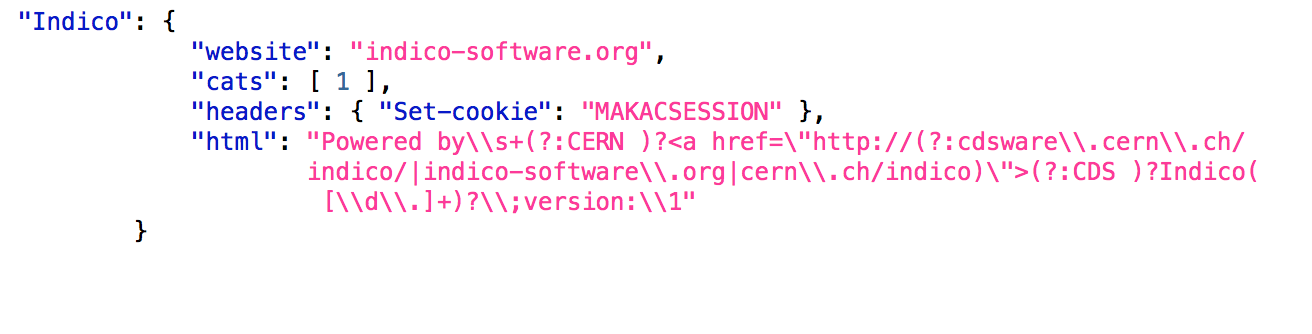
\includegraphics[width=1.0\textwidth]{indico}
  \caption{Indico Detection Rule}
  
\end{figure}
 
\subsubsection{WASDOM}

\label{wad_section}
wana talk abut pushing upstream?
\subsubsection{SSDB?}
\subsubsection{Auto-notify?}

***an image of the architecture: ssdb, autonotify, skipfish, nmap, etc.


\section{Objectives}
improving the current approaches
\begin{itemize}
\item each script its own format. there is a need for a wrapper that has a unique format, scripts can deal with only one resource and ... [scanner-> chapter]
\item missing vulnerabilties that do not create big noises in the public, manual check for wad outputs that match. Automate the monitoring of vulnerabilities to improve speed and accuracy of responding to vulnerabilities and automate the affected resource detection. [vunerability nitification tool -> chapter]

\item approaches for security, automated tools fo not discover everything
\end{itemize}

























